\documentclass[listings]{labreport}
\departmentsubject{Кафедра вычислительной техники}{Системное программное обеспечение}
\titleparts{Самостоятельная работа №1}{Знакомство с редактором vim}
\students{Лабушев Тимофей Михайлович}
\usepackage{multicol}
\usepackage{caption}
\usepackage{float}

\begin{document}

\maketitlepage

\section*{Введение. Редакторы vi и vim}

Отличительной чертой \texttt{vi} среди текстовых редакторов является модальность:
наличие нескольких режимов работы, в которых различается назначение клавиш
и, как следствие, возможные действия.

Редактор \texttt{vim} является развитием \texttt{vi} и включает в себя
множество возможностей, которые встречаются в современных редакторах, но
отсутствуют в \texttt{vi}: подсветка синтаксиса, язык скриптов и сторонние расширения,
разделение окна на панели и владки.

\section*{Режимы}

Как обозначено выше, определенные действия по редактированию текста
выполняются в определенных режимах. Основными являются:

\begin{itemize}
\item \textit{командный (command)}, также называемый \textit{нормальным (normal)}:
  вводимые символы интерпретируются как команды, которыми осуществляется навигация
  и производятся другие действия над текстом;
\item \textit{ввода (insert)}: вводимые символы вставляются в текст;
\item \textit{командной строки (command line)}: вводимые символы формируют
  командную строку для управления редактором (открытие и закрытие файлов,
  установка параметров).
\end{itemize}

В дополнение к ним, \texttt{vim} включает в себя \textit{визуальный (visual)} режим
для выделения текста. Команды нормального режима, применяемые к одному символу или линии,
будут применены ко всей выделенной области. 

\section*{Набор текста}

Ввод текста осуществляется в режиме \textit{insert}, переход в который осуществляется
следующими командами:

\begin{itemize}
\item \texttt{i}: вставить перед символом, на котором остановлен курсор;
\item \texttt{a}: вставить после символа, на котором остановлен курсор;
\item \texttt{I}: вставить в начало строки;
\item \texttt{A}: вставить в конец строки;
\item \texttt{o}: начать ввод на новой строке, вставленной после позиции курсора;
\item \texttt{O}: начать ввод на новой строке, вставленной перед позицией курсора.
\end{itemize}

Переход из режима \textit{insert} в \textit{normal} осуществляется с помощью
\texttt{ESC}.

\section*{Открытие и запись файлов}

По двоеточию \texttt{:}, нажатому в режиме \textit{normal}, происходит
переход к командной строке, в которую вводятся различные служебные команды,
в том числе для работы с файлами. Для выполнения базовых операций достаточно
следующих:

\begin{itemize}
\item \texttt{:w}, \texttt{:write}: записать изменения в файл;
\item \texttt{:w <file>}, \texttt{:write <file>}: создать новый файл
  по указанному пути и записать в него текст;
\item \texttt{:w! <file>}, \texttt{:write! <file>}: создать новый файл
  \textit{или перезатереть существующий} по указанному пути и записать в него текст;
\item \texttt{:e}, \texttt{:edit}: считать редактируемый файл с диска (чтобы
  отразить изменения, сделанные вне редактора), если в текущем нет несохраненных изменений;
\item \texttt{:e <file>}, \texttt{:edit <file>}: открыть для редактирования
  указанный файл, если в текущем нет несохраненных изменений;
\item \texttt{:e!}, \texttt{:e! <file>}, \texttt{:edit!}, \texttt{:edit! <file>}:
  считать файл, не сохраняя текущих изменений;
\item \texttt{:r <file>}, \texttt{:read <file>}: вставить текст из файла под курсором.
\end{itemize}

В отличии от большинства современных редакторов с заметной задержкой при запуске,
\texttt{vim} открывается достаточно быстро для стиля работы "запустить
редактор, отредактировать файл, закрыть редактор". Имя файла, который будет создан или изменен,
передается аргументом командной строки: \texttt{vim <file>}.

\section*{Навигация по тексту}

Посимвольное перемещение курсора влево, вправо, на строку вниз и на строку вверх
осуществляется командами \texttt{h, l, j, k} соответственно. Выбор обусловлен
конструкцией терминала, на котором изначально разрабатывался \texttt{vi}:

\begin{figure}[H]
  \begin{center}
  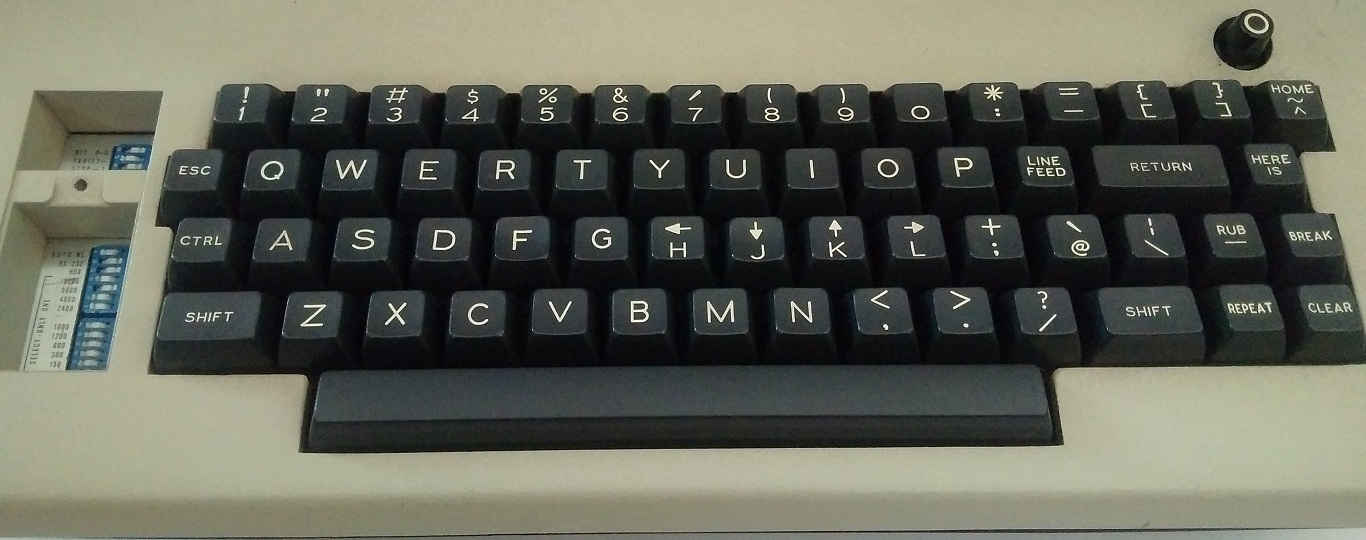
\includegraphics[width=0.85\textwidth, bb=0 0 1366 540]{vintagecomputer.ca-ADM3A.jpg}
  \captionsetup{labelformat=empty}
  \caption{\scriptsize Источник: https://vintagecomputer.ca/lear-siegler-adm-3a-terminal/}
  \end{center}
\end{figure}

В большинстве случаев удобнее перемещаться не по символам, а по словам. Для этого предназначены
команды \texttt{w} (перейти к началу следущего слова), \texttt{b} (вернуться к началу
предыдущего слова), \texttt{e} (перейти к концу слова).

Переход в конец строки происходит по команде \texttt{\$}, в начало — \texttt{0},
к первому символу после отступа — \texttt{\^{}}. Переход по параграфам осуществляется
командами \texttt{\{} (к предыдущему) и \texttt{\}} (к следующему).

Перемещение по файлу возможно с помощью комбинации \texttt{gg} (перейти в начало), команде
\texttt{G} (перейти в конец). Если перед \texttt{G} указать число, то выполнится переход на строку
с этим номером.

Числа могут предшествовать и другим командам, определяя число повторов. Например, \texttt{5w} перейдет
к пятому слову от текущей позиции, а \texttt{11j} переведет курсор на 11 строк ниже.

\section*{Операции над текстом}

Базовые:
\begin{itemize}
\item \texttt{yy}: скопировать строку;
\item \texttt{dd}: вырезать строку;
\item \texttt{p}: вставить после курсора (под курсором при вставке строки);
\item \texttt{P}: вставить перед курсором (над курсором при вставке строки);
\item \texttt{J}: присоединить следующую строку к текущей;
\item \texttt{u}: отменить последнее изменение.
\end{itemize}

Команды \texttt{y} (скопировать) и \texttt{d} (удалить) также применяются к:
\begin{itemize}
\item части текста (от символа до нескольких абзацев), выделенной в визуальном режиме;
\item части текста до вхождения символа справа (\texttt{f}) или слева (\texttt{F}) от курсора включительно
\item части текста до вхождения символа, не включая символ (\texttt{t} и \texttt{T});
\item одному или нескольким словам (\texttt{yw}, \texttt{d4w})
\end{itemize}

Примеры: \texttt{df.} удалит текст от положения курсора до точки, включая ее;
\texttt{y2t.} скопирует текст до второй точки, не включая ее.

\section*{Поиск и замена}

Приведенные выше команды \texttt{f}, \texttt{F}, \texttt{t}, \texttt{T}
позволяют искать символы лишь внутри строки.

Поиск по всему тексту инициируется командой \texttt{/}, за которой следует искомая строка.
Ввод завершается переходом на новую строку. Переход между результатами осуществляется
командами \texttt{n} (к следующему) и \texttt{N} (к предыдущему).

Для замены предназначены следующие варианты командной строки \texttt{:s}:
\begin{itemize}
\item \texttt{:s/search/replace/}: заменить первое вхождение \texttt{search} на \texttt{replace} в текущей строке;
\item \texttt{:s/search/replace/g}: заменить все вхождения \texttt{search} на \texttt{replace} в текущей строке;
\item \texttt{:\%s/search/replace/}: заменить первое вхождение \texttt{search} на \texttt{replace} в каждой строке;
\item \texttt{:\%s/search/replace/g}: заменить все вхождения \texttt{search} на \texttt{replace} в тексте.
\end{itemize}

\section*{Работа с несколькими файлами}

Несколько файлов могут быть открыты с помощью \texttt{:e}. Для отображения открытых файлов используется
командная строка \texttt{:ls}, переход между ними осуществляется командой \texttt{:b <file>}.

Рабочее пространство может быть разделено на несколько окон командными строками \texttt{:sp} и \texttt{:vs}.
Первая разместит новое окно горизонтально, вторая — вертикально. Переключение между окнами осуществляется
сочетанием \texttt{Ctrl-W w}.

В новых версиях \texttt{vim} рабочее пространство разделяется не только на окна, но и на вкладки,
каждая из которых может содержать несколько окон. \texttt{:tabnew} создает пустую вкладку,
\texttt{:tabe <file>} открывает в новой вкладке файл, \texttt{:tabnext} и \texttt{:tabprevious}
переходят между вкладками.

\section*{Изменение параметров редактора}

В домашней директории пользователя может быть размещен файл \texttt{.vimrc} (\texttt{.exrc} для \texttt{vi})
с командными строками, которые будут исполнены при открытии редактора.

Для установки большинства опций редактора используется \texttt{:set}. Пример показа/сокрытия номеров строк:
\begin{itemize}
\item \texttt{set number}: показывать номера строк;
\item \texttt{set nonumber}: скрыть номера строк;
\item \texttt{set number?}: вывести текущее значение опции (\texttt{number} или \texttt{nonumber}).
\end{itemize}

Опция \texttt{list} позволяет отображать специальные символы.

\section*{Выход из редактора}

Для выхода из \textit{vi(m)} предназначены следующие командные строки:

\begin{itemize}
\item \texttt{:q}, \texttt{:quit} — выйти, если нет несохраненных изменений;
\item \texttt{:q!}, \texttt{:quit!} — выйти без сохранения изменений;
\item \texttt{:wq} — записать файл и выйти;
\item \texttt{:x} — записать файл, если есть несохраненные изменения, и выйти.
\end{itemize}

\end{document}
